\documentclass{article}

\usepackage{tikz}
\usetikzlibrary{automata,shapes}

\usepackage{charter}

\begin{document}
				
\begin{figure}
\begin{center}
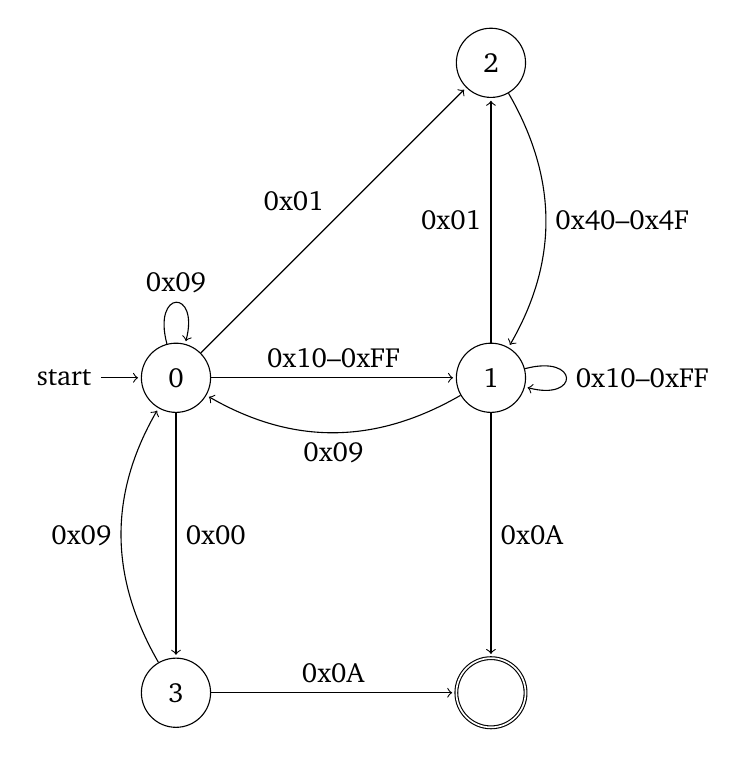
\begin{tikzpicture}[shorten >=1pt,auto, node distance=4cm]
	\node[state,initial]	(q0)	{0};
	\node[state]		(q1) [right of=q0]	{1};
	\node[state]		(q2) [above of=q1]	{2};
	\node[state]		(q3) [below of=q0]	{3};
	\node[state,accepting]	(q4)	[below of=q1]	{};
	\path[->]
		(q0)	edge				node {0x01}		(q2)
			edge 			node {0x10--0xFF}	(q1)
			edge				node {0x00}		(q3)
			edge [loop above] 	node {0x09}		(q0)
		(q2)	edge [bend left] 	node {0x40--0x4F}	(q1)
		(q1) 	edge 			node {0x01} 		(q2)
			edge [bend left] 	node {0x09} 		(q0)
			edge [loop right] 	node {0x10--0xFF} 	(q1)
			edge				node {0x0A}		(q4)
		(q3)	edge	[bend left] 	node {0x09}		(q0)
			edge  			node {0x0A}		(q4)
		;
\end{tikzpicture}
\end{center}
\caption{Finite-State Machine for HandlerSocket Protocol}
\end{figure}

\end{document}
